\chapter{Montaje del robot}
\label{cap:montajedelrobot}
En este capítulo se describirá la estructura que hemos compuesto con las barras y las bases del robot para que este se adaptara a las necesidades del proyecto. Para controlar nuestro robot de una forma más cómoda se le dotó de una \textit{Raspberry Pi} que hará de puente entre nuestro ordenador, en el que lanzaremos los nodos necesarios para el completo funcionamiento del sistema de navegación, y el robot ya que los conectará vía WIFI, esto se explicará más en detalle en el apartado de Diseño de conectividad. Por último se expondrá el modelo de Gazebo creado para nuestro robot, el cual nos ayudará a simular el robot real de la mejor forma posible .

\section{Estructura}
\label{cap:estructuradelrobot}
La estructura establecida consta de:
\begin{enumerate}
\item Base móvil. Es la base por defecto del robot Kobuki. Sobre esta base se colocará la batería que alimentará a la \textit{Raspberry Pi} y algunos reductores de voltaje o tensión para poder adecuar las tensiones de salida del robot con las tensiones de entrada de los componentes que compondrán la parte hardware
\item Plataforma. Anclada a la base móvil por 4 pequeñas barras metálicas situaremos una primera plataforma. Con ella cubriremos muchos cables, la batería externa y algunos componentes electrónicos, proporcionándoles protección y evitando que se vean. Sobre esta colocaremos un hub usb y nuestra Raspberry Pi. 
\item Segunda plataforma. Anclaremos esta segunda plataforma a la primera con barras metálicas, esta vez más largas. Sobre ella colocaremos nuestro sensor láser, de esta manera el sensor no se verá obstaculizado por ningún objeto como pudiera ser las barras metálicas.
\end{enumerate}

\section{Diseño de conectividad}
\label{cap:conectividad}
Se optó por un diseño de conectividad distribuido, aprovechando así el modelo distribuido que nos ofrece ROS, para vencer las dificultades e incomodidades de tener que poner nuestro ordenador encima del robot y este conectado directamente al él, como se estaba haciendo hasta ahora. En este nuevo modelo será una Raspberry Pi la que esté conectada al robot, creará un Access Point y nosotros nos conectaremos a este AP para lanzar nuestro sistema de navegación. De esta manera la Raspberry Pi se convierte en un mero puente para la información del robot y de los sensores entre el robot y nuestro ordenador. Conseguimos así poder ejecutar pruebas o depurar nuestro algoritmo de una manera más cómoda y sencilla. 

Los requisitos con los que tiene que contar nuestra Raspberry Pi son los siguientes:
\begin{itemize}
\item \textbf{Raspberry Pi 2 Model B.} Para poder instalar el sistema operativo necesario y contar con un mínimo aceptable de capacidad de cómputo, memoria RAM y puertos USB, el primer requisito es contar con una placa del modelo mencionado, aunque puede ser también superior.
\item \textbf{Ubuntu 14.04 y ROS Indigo.} La distribución sobre la que trabajaremos tanto en el ordenador como en la Raspberry Pi será ROS Indigo, asociada a la distribución de Ubuntu 14.
\item \textbf{Alimentación.} Raspberry Pi puede alimentarse directamente con un transformador enchufado a la corriente, pero en nuestro caso, para evitar tener cables y que el robot sea totalmente autónomo, se necesitará una batería externa. En nuestro caso usamos un Power Bank de xxxxx mAh.
\item \textbf{Módulo WIFI.} La placa elegida no cuenta con módulo por defecto por lo que será necesario conectarle un módulo externo USB.
\item \textbf{Tarjeta de memoria.} Raspberry Pi necesita una tarjeta de memoria externa para poder funcionar. En nuestro caso usaremos una de xxxx GB. Esta capacidad es suficiente para albergar el SO, la distribución de ROS y los drivers del robot y los sensores.
\end{itemize}



\section{Modelo de Gazebo}
\label{cap:modelodegazebo}
Para crear un modelo fidedigno del robot real en el simulador Gazebo se utilizaron las medidas del robot real. Se tuvo en cuenta la altura respecto al suelo, la inclinación y profundidad de elementos críticos, como el láser, y se modificó el modelo por defecto de kobuki que se tiene en ROS para crear nuestro propio modelo de robot.

\begin{figure} [hbtp]
  \begin{center}
    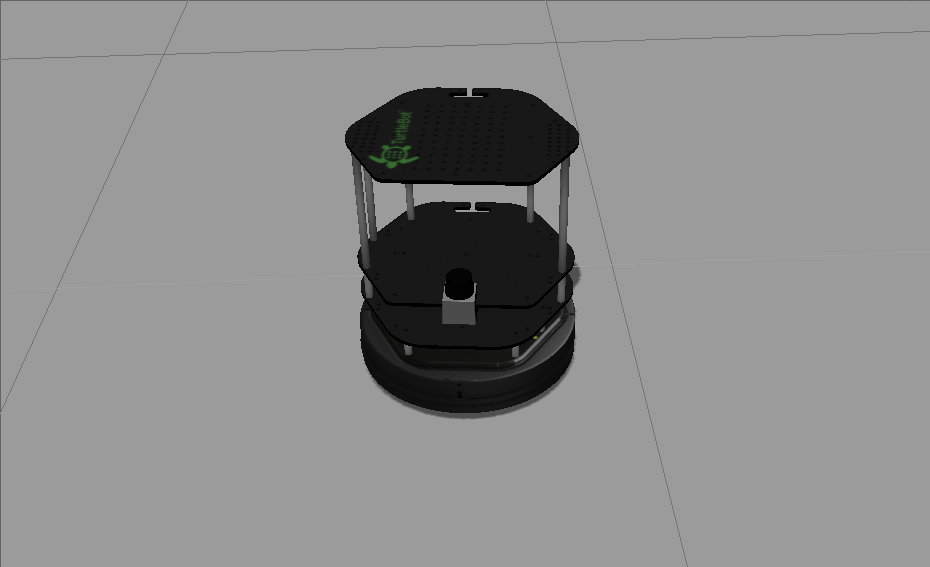
\includegraphics[width=9cm]{img/cap4/modelogazebo}
  \end{center}
  \caption{Visualización del modelo de robot de Gazebo.}
  \label{fig:modelogazebo}
\end{figure}


Es muy importante que el modelo se ajuste lo máximo posible a la realidad ya que muchas de las pruebas se realizarán en el simulador en primera instancia y más tarde se llevarán al robot real.
